%%%%%%%%%%%%%%%%%%%%%%%%%%%%%%%%%%%%%%%%%%

\section{Results of the cut-based analysis}

\label{sec:results}

In this section we present the results of the 
cut-based analysis, including the corresponding
cut-flow.
We
compare our results with other recent studies,
and in particular
we study how the signal significance
is affected if only the $4b$ component of the
QCD multi-jet background is taken into account,
while the $2b2j$ and $4j$ components are neglected.
%


\subsection{Cut-flow and signal significance}

First of all, we compare the cross-sections at various
analysis levels for the three categories, for signal and background events,
by providing a detailed cut-flow.
%
We consider all backgrounds enumerated in Sect.~\ref{mcgeneration},
and also discuss how results are modified if only the $4b$
component is kept.
%
At each stage of the cut-flow, we also provide the
the signal significance, $S/\sqrt{B}$, and the signal
over background ratio, $S/B$, corresponding to the
 HL-LHC with
an integrated luminosity of $\mathcal{L}
=3000$ fb$^{-1}$.
%
For this type of analysis,
it is crucial not only to achieve a good signal
significance, $S/\sqrt{B}$, but also a good signal over background ratio $S/B$.
%
If the latter is too small, an unrealistically precise
measurement of the background would be required.
%
In Table~\ref{tab:cutflowdetails}
we describe this cut-flow,
separated into the (exclusive) boosted, intermediate,
    and resolved categories.
    %
    From top to bottom, additional cuts are required in addition
    to the previous ones.
    %
    The various cuts
    are defined as follows:

   

%%%%%%%%%%%%%%%%%%%%%%%%%%%%%%%%%%%%%%%%%%%%%%%%%%%%%%%%%%%%%%%%%%%%%%%%%%%%%%%%%%%%%%%%%
%%%%%%%%%%%%%%%%%%%%%%%%%%%%%%%%%%%%%%%%%%%%%%%%%%%%%%%%%%%%%%%%%%%%%%%%%%%%%%%%%%%%%%%%%
\begin{table}[t]
  \centering
  \begin{tabular}{|c|c|c|c|}
\hline
&  Boosted  &   Intermediate &  Resolved  \\
\hline
\hline
{\bf C0} &  \multicolumn{3}{c|}{Generator level} \\
\hline
{\bf C1a} & $N_{\rm jets}^{R10}\ge 2$ & $N_{\rm jets}^{R04}\ge 2$, $N_{\rm jets}^{R10}=1$  &
$N_{\rm jets}^{R04}\ge 4$ \\
\hline
{\bf  C1b} & \multicolumn{3}{c|}{+$p_T$ cuts} \\
{\bf C1c} & \multicolumn{3}{c|}{+rapidity cuts}\\
\hline
 {\bf C1d} & +$N_{\rm MDT}\ge 2$ & +$N_{\rm jets}^{R10}=1$ with MDT  &
 +Higgs reconstruction \\
 \hline
{\bf C1e} & \multicolumn{3}{c|}{ +$m_H$ window cut} \\
\hline
{\bf C2} & \multicolumn{3}{c|}{+$b$-tagging}    \\
\hline
  \end{tabular}
  \caption{\small Cut-flow of the present analysis for the boosted, intermediate
    and resolved selections.
    %
      \label{tab:cutflowdetails}
  }
\end{table}
%%%%%%%%%%%%%%%%%%%%%%%%%%%%%%%%%%%%%%%%%%%%%%%%%%%%%%%%%%%%%%%%%%%%%%%%%%%%%%%%%%%%%%%%%
%%%%%%%%%%%%%%%%%%%%%%%%%%%%%%%%%%%%%%%%%%%%%%%%%%%%%%%%%%%%%%%%%%%%%%%%%%%%%%%%%%%%%%%%%


    \begin{itemize}
    \item {\bf C0}: these are the generator level cross-sections, with
      mild generation cuts in the case of the background processes, and no
      generation cuts
      for the signal events.
      %
    \item {\bf C1a}:  we only check that we have at least
      two large-$R$ jets (in the boosted case),
      one large-$R$ jet and at least 2 small-$R$ jets (in the intermediate
      case) and at least four small-$R$ jets (in the resolved case).
      %
      No acceptance requirements are imposed.
    \item {\bf C1b}: require that the above jets should
      satisfy the corresponding $p_T$ thresholds,
      $p_T \ge 200$ GeV for large-$R$ jets and
      $p_T \ge 50$ GeV for small-$R$ jets.
    \item {\bf C1c}: same for the
      rapidity acceptance requirement.
    \item {\bf C1d}: the two leading large-$R$ jets must
      be mass-drop tagged in the boosted category.
      %
      In the intermediate category, the large-$R$ jet must also be mass-drop tagged.
      %
    \item {\bf C1e}: after the two Higgs candidates  have been reconstructed,
      their invariant masses are required to lie a window around $m_H$,
      in particular between 85 and 165 GeV.
          \item {\bf C2}: finally, the
            $b$-tagging conditions are
            imposed, see
            Sect.~\ref{sec:btagging}.
      \end{itemize}
    Signal and background events satisfying all the analysis cut up to the
    C2 level
    are then used as input for the MVA training, to be described next
    in Sect.~\ref{sec:mva}.

    %
    In Table~\ref{tab:cutflow_noPU_1} we provide
    the values of cross-sections, in femtobarns,
     for the signal
      and the various background
      components as a function of the
      cut-flow, for the resolved,
      boosted and intermediate
      categories.
      %
       In each case, we also provide the signal over
      background ratio, $S/B$, and the signal
      significance, $S/\sqrt{B}$, at the HL-LHC, considering either
      the total background or only the $4b$ component.
     %
      This separation emphasizes
      the  importance of the reducible component of the QCD background.
      %
      Even after $b$-tagging, the reducible $2b2j$ background
      is comparable, or even larger, than the irreducible
      $4b$ component.
      %
      %
      So at the end of the cut-based analysis, signal significance
      are overestimated by up to a factor 2 if the light
      and charm jet background is neglected.

      
    

%%%%%%%%%%%%%%%%%%%%%%%%%%%%%%%%%%%%%%%%%%%%%%%%%
\begin{table}[t]
  \centering
  \scriptsize
  \begin{tabular}{|l|cc|cccc|cccc|}
  \hline
\multicolumn{11}{|c|}{Resolved category, $\la n_{\rm PU}\ra=0$}\\
\hline
&  \multicolumn{6}{c|}{Cross-section [fb]} &  &  & &  \\
   &  $hh\to 4b$ &  total bkg  &   $4b$    &  $2b2j$   &   $4j$    &
$t\bar{t}$ &
$S/B_{\rm tot}$ & $S/B_{\rm 4b}$ & $S/\sqrt{B_{\rm tot}}$ & $S\sqrt{B_{\rm 4b}}$ \\
  \hline
  \hline
 C0    & $39$  &   $5.2\cdot 10^9$   & $1.8\cdot 10^6$ & $3.5\cdot 10^8$ & $4.9\cdot 10^9$ & $3.5\cdot 10^5$  & $7.5\cdot 10^{-9}$   &  $2.2\cdot 10^{-5}$  &   0.03   & 1.6        \\
 C1a   & $39$  &   $5.2\cdot 10^9$   & $1.8\cdot 10^6$ & $3.5\cdot 10^8$ & $4.9\cdot 10^9$ & $3.5\cdot 10^5$ &  $7.5\cdot 10^{-9}$   & $2.2\cdot 10^{-5}$   &     0.03   & 1.6       \\
 C1c   & $22$  &   $2.2\cdot 10^8$   & $6.9\cdot 10^4$ & $1.5\cdot 10^7$ & $2.0\cdot 10^8$ & $2.1\cdot 10^5$ &  $1.0\cdot 10^{-7}$  &  $3.2\cdot 10^{-4}$  &  0.08   & 4.6         \\
 C1d   & $22$  &   $2.2\cdot 10^8$   & $6.9\cdot 10^4$ & $1.5\cdot 10^7$ & $2.0\cdot 10^8$ & $2.1\cdot 10^5$ &  $1.0\cdot 10^{-7}$  & $3.2\cdot 10^{-4}$   &  0.08   & 4.6         \\
 C1e   & $63$  &   $4.4\cdot 10^7$   & $1.6\cdot 10^4$ & $3.2\cdot 10^6$ & $4.1\cdot 10^7$ & $8.8\cdot 10^4$ &   $1.4\cdot 10^{-7}$  &  $3.9\cdot 10^{-4}$   &   0.05   & 2.7         \\
 C2    & $1.2$  &   $4.9\cdot 10^3$   & $1.7\cdot 10^3$ & $2.9\cdot 10^3$ & $2.1\cdot 10^2$ & $47$ &            $ 2.5\cdot 10^{-4}$   & $7.1\cdot 10^{-4}$   &   0.97   & 1.6       \\
\hline
\end{tabular}

  $\,$ \\
  \vspace{0.5cm}
  \begin{tabular}{|l|cc|cccc|cccc|}
  \hline
\multicolumn{11}{|c|}{Intermediate category}\\
\hline
&  \multicolumn{6}{c|}{Cross-section [fb]} &  &  & &  \\
   &  $hh\to 4b$ &  total bkg  &   $4b$    &  $2b2j$   &   $4j$    &
$t\bar{t}$ &
$S/B_{\rm tot}$ & $S/B_{\rm 4b}$ & $S/\sqrt{B_{\rm tot}}$ & $S\sqrt{B_{\rm 4b}}$ \\
  \hline
  \hline
 C0      & 39  &   $5.2\cdot 10^9$   & $1.8\cdot 10^6$ & $3.5\cdot 10^8$ & $4.9\cdot 10^9$ & $3.5\cdot 10^5$ &  $7.5\cdot 10^{-9}$   & $2.2\cdot 10^{-5}$   &   $3.0\cdot 10^{-2}$   & 1.6  \\
 C1c     & 6.9  &   $8.4\cdot 10^7$   & $2.1\cdot 10^4$ & $5.3\cdot 10^6$ & $7.9\cdot 10^7$ & $3.3\cdot 10^4$ &  $8.2\cdot 10^{-8}$   & $3.3\cdot 10^{-4}$ &   $4.1\cdot 10^{-2}$   & 2.6 \\
 C1d     & 6.3  &   $5.8\cdot 10^7$   & $1.4\cdot 10^4$ & $3.6\cdot 10^6$ & $5.5\cdot 10^7$ & $3.0\cdot 10^4$ &  $1.1\cdot 10^{-7}$   & $4.6\cdot 10^{-4}$ &   $4.5\cdot 10^{-2}$   & 2.9\\
 C1e     & 1.3  &   $3.5\cdot 10^6$   & $8.7\cdot 10^2$ & $2.1\cdot 10^5$ & $4.3\cdot 10^7$ & $8.8\cdot 10^3$ &  $3.8\cdot 10^{-7}$   & $1.5\cdot 10^{-3}$  &   $3.9\cdot 10^{-2}$   & 2.5\\
 C2      & 0.22  &   $1.8\cdot 10^2$   & $5.6\cdot 10^1$ & $9.6\cdot 10^1$ & $2.2\cdot 10^1$ & 3.1 & $1.3\cdot 10^{-3}$   & $4.0\cdot 10^{-3}$  &   $9.2\cdot 10^{-1}$   & 1.6 \\
\hline
\end{tabular}

  $\,$ \\
  \vspace{0.5cm}
    \begin{tabular}{|l|cc|cccc|cccc|}
  \hline
\multicolumn{11}{|c|}{Boosted category, $\la n_{\rm PU}\ra=0$}\\
\hline
&  \multicolumn{6}{c|}{Cross-section [fb]} &  &  & &  \\
   &  $hh\to 4b$ &  total bkg  &   $4b$    &  $2b2j$   &   $4j$    &
$t\bar{t}$ &
$S/B_{\rm tot}$ & $S/B_{\rm 4b}$ & $S/\sqrt{B_{\rm tot}}$ & $S\sqrt{B_{\rm 4b}}$ \\
  \hline
  \hline
C0      & 39  &   $5.2\cdot 10^9$   & $1.8\cdot 10^6$ & $3.5\cdot 10^8$ & $4.9\cdot 10^9$ & $3.5\cdot 10^5$  &   $7.5\cdot 10^{-9}$   & $2.2\cdot 10^{-5}$  &  $ 3.0\cdot 10^{-2}$   & 1.6 \\
 C1a     & 39  &   $5.2\cdot 10^9$   & $1.8\cdot 10^6$ & $3.5\cdot 10^8$ & $4.9\cdot 10^9$ & $3.5\cdot 10^5$  &   $7.5\cdot 10^{-9}$   & $2.2\cdot 10^{-5}$ &  $ 3.0\cdot 10^{-2}$   & 1.6  \\
 C1c     & 9.4  &   $4.6\cdot 10^7$   & $1.1\cdot 10^4$ & $2.9\cdot 10^6$ & $4.3\cdot 10^7$ & $2.4\cdot 10^4$ &   $2.0\cdot 10^{-7}$   & $8.3\cdot 10^{-4}$ &  $ 7.6\cdot 10^{-2}$   & 4.8 \\
 C1d     & 6.7  &   $3.7\cdot 10^7$   & $7.5\cdot 10^3$ & $2.1\cdot 10^6$ & $3.5\cdot 10^7$ & $2.2\cdot 10^4$ &   $1.8\cdot 10^{-7}$   & $9.0\cdot 10^{-4}$ &  $ 6.0\cdot 10^{-2}$   & 4.2  \\
 C1e     & 2.5  &   $3.9\cdot 10^6$   & $8.0\cdot 10^2$ & $2.3\cdot 10^5$ & $3.7\cdot 10^6$ & $7.1\cdot 10^3$   &   $6.4\cdot 10^{-7}$   & $3.1\cdot 10^{-3}$ &  $ 6.9\cdot 10^{-2}$   & 4.9\\
 C2      & 0.4  &   $2.5\cdot 10^2$   & $5.3\cdot 10^1$ & $1.9\cdot 10^2$ & $1.3\cdot 10^1$ & 1.6  &   $1.4\cdot 10^{-3}$   & $6.7\cdot 10^{-3}$ &   1.2   & 2.7  \\
\hline
\end{tabular}
%%%%%%%%%%%%%%%%%%%%%%%%%%%%%%%%%%%%%%%%%%%%%%%%%%%%%%%%%%%%%%%

    \caption{\small The cross-sections, in femtobarns,
      for the signal and the various background
      processes at different steps of the
      cut-flow, for the resolved (upper table),
      intermediate (middle table) and boosted
      (lower table) categories, for the analysis
      without PU.
      %
      In each case, we also provide the signal over
      background ratio, $S/B$, and the signal
      significance, $S/\sqrt{B}$, considering either
      the total background or only the $4b$ component.
      %
      The different levels of the cut-flow are summarized
      in Table~\ref{tab:cutflowdetails}.
 \label{tab:cutflow_noPU_1}}
\end{table}
%%%%%%%%%%%%%%%%%%%%%%%%%%%%%%%%%%%%



%
In the boosted category, after all cuts,
one ends
up with more than 1K signal events expected
at the HL-LHC, swamped  however in a almost 1M background events,
leading to $S/\sqrt{B}=1.2$ and $S/B=0.0014$.
%
It should have been possible to somewhat increase this significance
but using more aggressive cuts,
but this is not needed due to the subsequent
optimisation  performed with the MVA.
%
From  Table~\ref{tab:cutflow_noPU_1}
it is also possible to compute the corresponding pre-MVA
expectations for the LHC Run II with
$\mathcal{L}=300$ fb$^{-1}$: one expects
120 signal events, with signal significance dropping down to
$S/\sqrt{B}\sim 0.3$.
%

Both the intermediate and resolved categories benefit from higher signal yields,
specially in the resolved category, but this enhancement is compensated by the
corresponding
increase in the QCD multi-jet background.
%
In both categories
the signal significance is similar to that of the boosted category,
$S\sqrt{B}=0.97(0.92)$ in the resolved
(intermediate) categories,
with the drawback, in the resolved case,
that $S/B$
is one order to magnitude smaller.
%
Combining the pre-MVA results
from the
of the boosted, intermediate and resolved categories,
we obtain a significance for the observation of the Higgs pair production
in the $b\bar{b}b\bar{b}$ final
state at the HL-LHC of  $S/\sqrt{B}=1.8$.

\subsection{The role of light  and charm jet mistags}

One of the main differences of the present study as compared
to previous works is the inclusion of both irreducible
and reducible background components, which allows
to study the impact of the modeling of light and charm jet mistags. 
%
Two recent studies that have also studied the
feasibility of SM Higgs pair production in the $b\bar{b}b\bar{b}$
final state are from the UCL group~\cite{Wardrope:2014kya} and from
the
Durham group~\cite{deLima:2014dta}.
%
The UCL study based
on requiring at least four $b$-tagged $R=0.4$ anti-$k_T$ jets
in central acceptance with $p_T \ge 40$ GeV, which are
then used to construct dijets (Higgs candidates) with
$p_T \ge 150$ GeV, $85 \le m_{\rm dijet} \le 140$ GeV
and $\Delta R \le 1.5$ between the two components
of the dijet.
%
In addition to the basic selection cuts, the discriminating
power of
additional variables is included by means of a 
Boosted Decision Tree (BDT) discriminant.
%
The backgrounds included are the $4b$ and
$2b2c$ QCD multijets, as well as
$t\bar{t}$, $Zh$, $t\bar{t}h$ and $hb\bar{b}$,
and a signal significance of $S/\sqrt{B}=2.1$ for the HL-LHC
is obtained.

The Durham group study~\cite{deLima:2014dta} requires events
to have two $R=1.2$ C/A jets with $p_T\ge 200$ GeV, with
two $b$-tagged subjets inside each large-$R$ jet with
$p_T \ge$ 40 GeV each.
%
To improve the separation between
signal over background separation, both the BDRS
method and the Shower Deconstruction (SD)~\cite{Soper:2011cr,Soper:2012pb}
technique are used.
%
The background considered are QCD $4b$ as well as $Zb\bar{b}$, $hZ$ and
$hW$.
%
At the HL-LHC, the best result is obtained by requiring two
SD-tagged large-$R$ jets, which leads to $S/\sqrt{B}\sim 2.1$, with
 slightly inferior performance with the BDRS tagger.
 %
 

%
 From the results of Table~\ref{tab:cutflow_noPU_1}, we observe
 that the signal significance in the boosted, intermediate,
 and resolved categories is 2.7, 1.6 and 1.6 respectively,
 when only the QCD $4b$ background is included.
 %
 Combining the signal significance in the three categories,
 we
 obtain  a total $S/\sqrt{B_{\rm 4b}}=3.5$, which is a factor
 2 improvement as compared to the result found when
 all background components are included.
 %
 This should be taken into account when comparing
 the results of this work with previous analysis.
 %

 It is interesting to compare in each category the interplay
 between the reducible and irreducible components of the
 QCD backgrounds.
 %
 In the resolved case, the $4b$ and $2b2j$ have a similar
 magnitude, with the latter being larger by a factor of two,
 with $4j$ being smaller by an order of magnitude.
 %
 The situation is similar in the intermediate category, while
 in the boosted category the importance of the $2b2j$ component
 is even more marked, being a factor four larger than the
 $4b$ one.
 %
 Therefore, we conclude that, while the $4j$ component can be safely
 neglected (given the theory uncertainties associated to the
 modelling of the QCD background), the inclusion of the
 $2b2j$ component is essential to robustly assess the feasibility
 of measuring Higgs pairs in this final state.
 %
 This indicates that a promising avenue to improve the prospects
 of this measurement would be to reduce, as much as possible,
 the light and charm jet mistag rate, in addition to achieving
 a higher $b$-tag efficiency.


 In Fig.~\ref{fig:histoBack} we show a
 comparison
    of the shapes of the $4b$ and $2b2j$
components of the QCD background for the $p_T$ of the leading
Higgs candidate in the resolved
and boosted  categories, and the same
 for the invariant
mass $m_{hh}$ of the
    reconstructed di-Higgs system.
    %
    The two components lead to a rather similar shape
    for the two distributions, with some interesting
    differences, for instance in the boosted
    category the $4b$ component is harder for the
    $p_T^h$ distribution, while the $2b2j$ leads to a longer
    tail at small values of the $m_{hh}$ invariant
    mass distribution.
%
    We also observe that the $2b2j$ distributions
    are affected by somewhat larger
    MC fluctuations as compared to $4b$, despite the large size
of the initial sample.
%
This is a consequence of the
difficulties of an accurate modelling of the effects
of $b$-jet mistags from a QCD multi-jets process, requiring
very large MC samples.

%%%%%%%%%%%%%%%%%%%%%%%%%%%%
\begin{figure}[t]
\begin{center}
 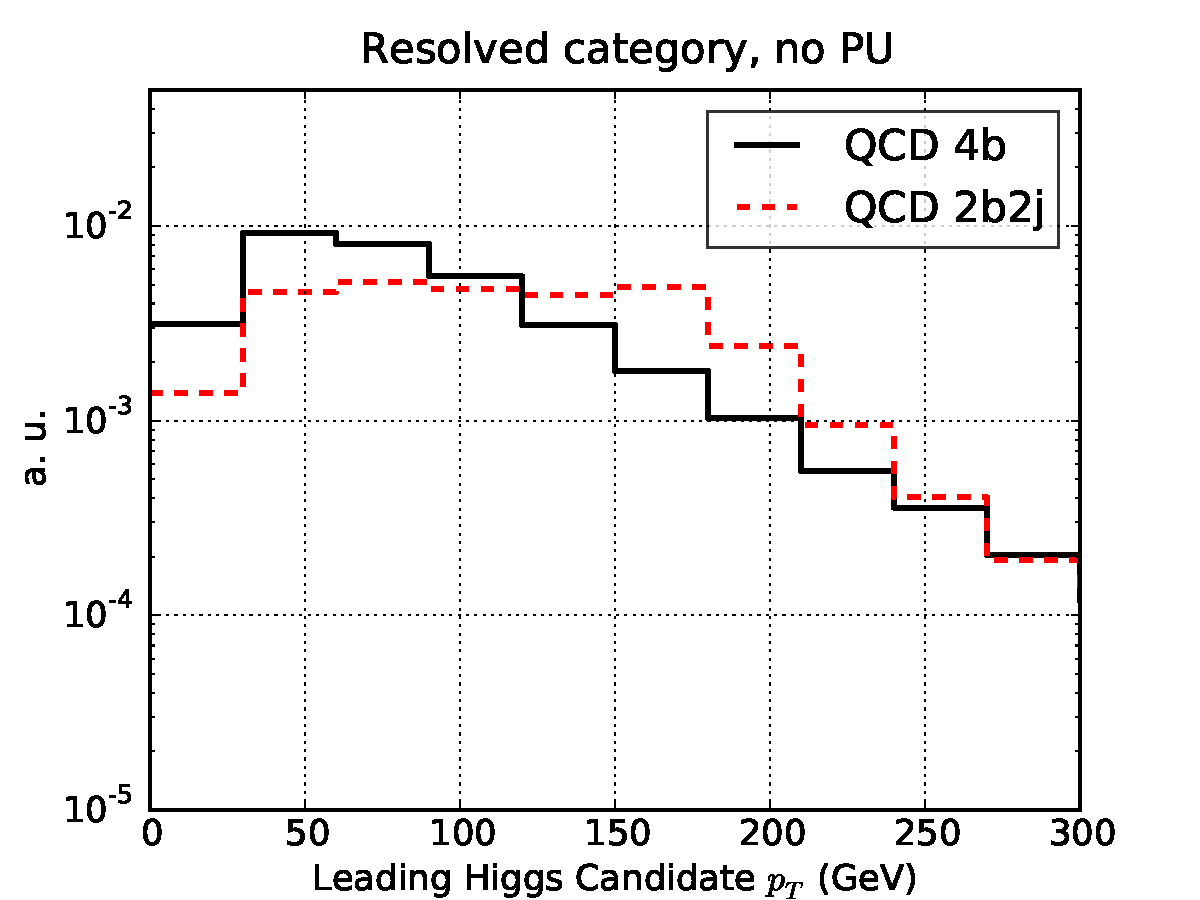
\includegraphics[width=0.49\textwidth]{plots/pt_h0_C2_res_back_noPU.pdf}
 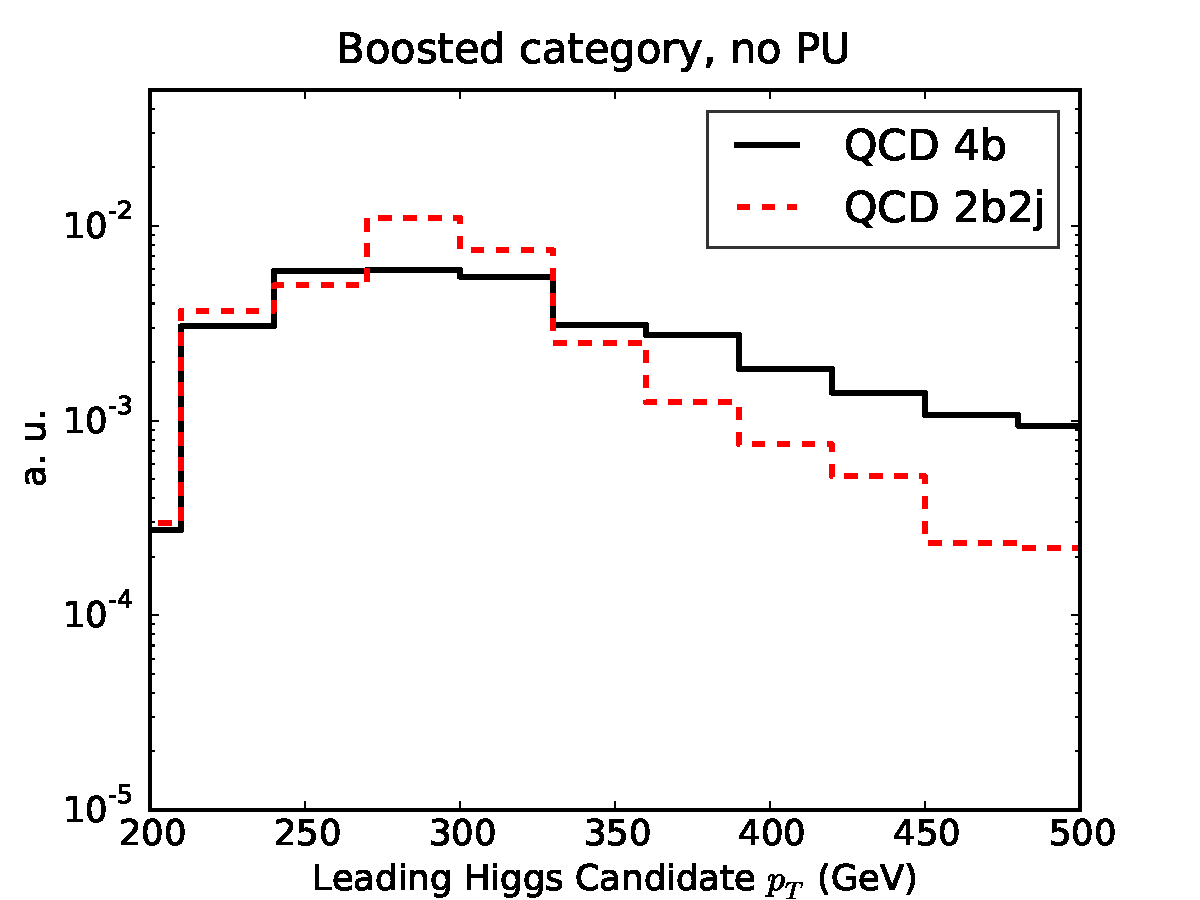
\includegraphics[width=0.49\textwidth]{plots/pt_h0_C2_bst_back_noPU.pdf}
  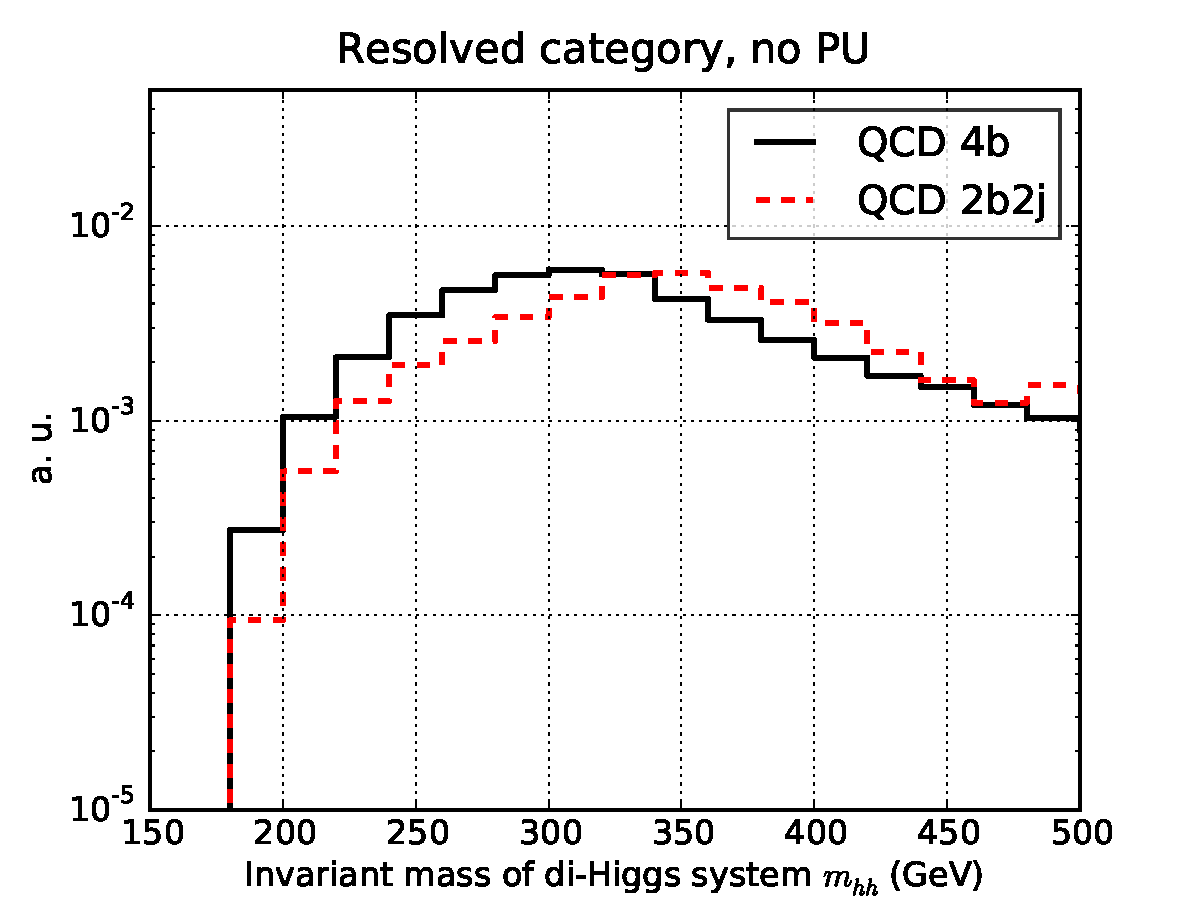
\includegraphics[width=0.49\textwidth]{plots/m_hh_C2_res_back_noPU.pdf}
  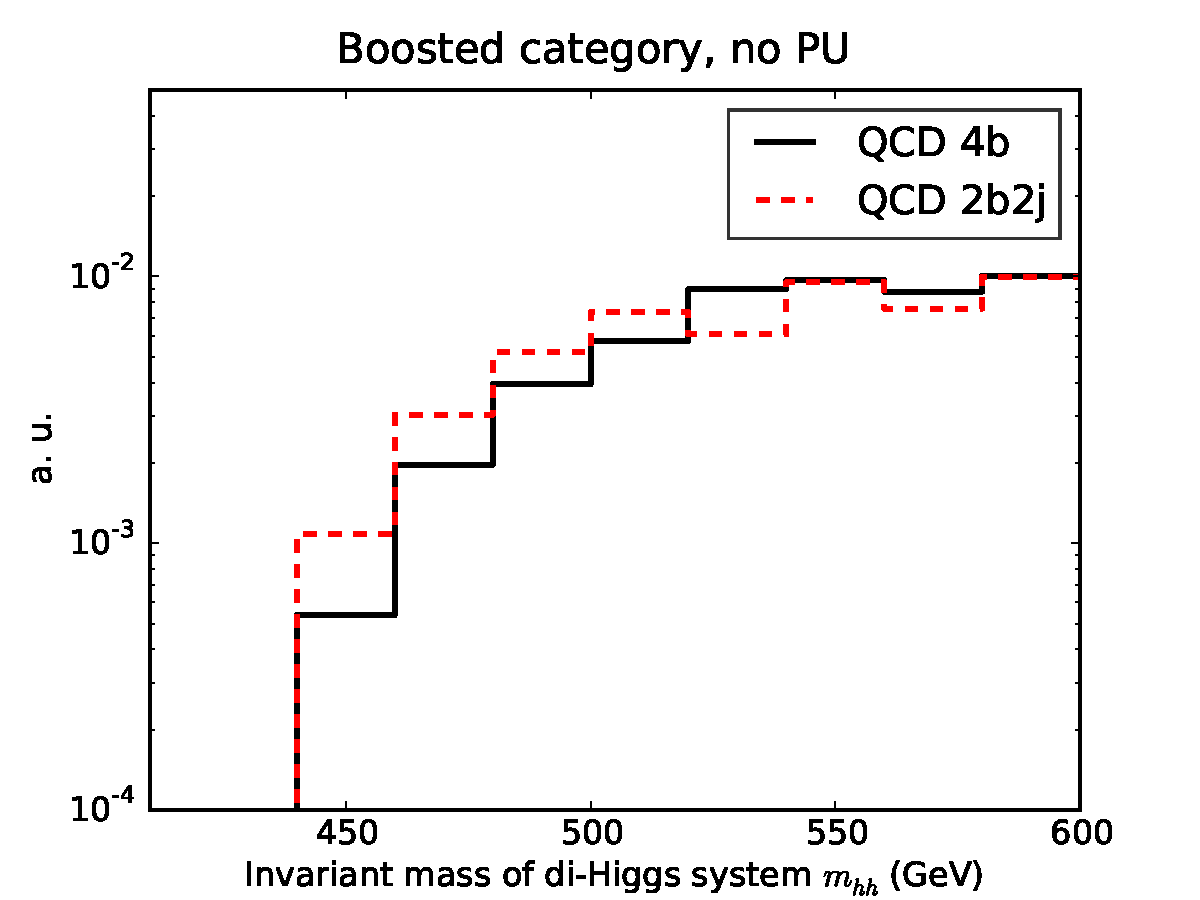
\includegraphics[width=0.49\textwidth]{plots/m_hh_C2_bst_back_noPU.pdf}
  \caption{\small
    Upper plots: comparison
    of the shapes of the $4b$ and $2b2j$
components of the QCD background for the $p_T$ of the leading
Higgs candidate in the resolved
(left plot) and boosted (right plot) categories.
    %
Lower plots: the same comparison this time for the invariant
mass $m_{hh}$ of the
    reconstructed di-Higgs system.
}
\label{fig:histoBack}
\end{center}
\end{figure}
%%%%%%%%%%%%%%%%%%%%%%%

The reason why the  $2b2j$ process
is not negligible as compared to the $4b$ component
is the following.
%
In the boosted category, for example,
the cross-sections at the C1e
level, that is, after the mass-drop tagging but before
$b$-tagging, is a factor 300 larger in the $2b2j$
sample as compared to the $4b$ sample.
%
Now, after $b$-tagging, the naive expectation would
be a suppression of the former by a factor $f_l^2 =10^{-4}$,
since a total of four $b$-tags are required to classify the
event as a Higgs candidate.
%
So the ratio of $2b2j$ over $4b$ should be
around $\simeq 3\%$.
  %
While  we have checked that this expectation is borne
out at parton level, before showering,
we find that  when parton shower effects
are accounted for, due to the radiation of $b\bar{b}$ pairs from the
light jets as well as due to combinatorics, the
number of  $b$ quarks in the  final state is
increased substantially in the $2b2j$ component as compared
to the parton level content,
enhancing the signal efficiency and making
it comparable to the $4b$ component.


